To investigate the efficacy of Roots as an approach to
implementing performance diagnostics as a PaaS service, we have developed a
working prototype, and a set of algorithms that uses it to automatically
identify SLO-violating performance anomalies.
For this investigation, we integrate Roots into AppScale~\cite{6488671}, an open source PaaS cloud
that is API-compatible with the Google App Engine~\cite{gae} public cloud.  
AppScale can run on bare metal or within cloud infrastructures (Amazon EC2, Eucalyptus, 
etc.), and executes GAE applications without modification.
We minimally modify AppScale's internal components to integrate Roots.

\begin{figure}
\centering
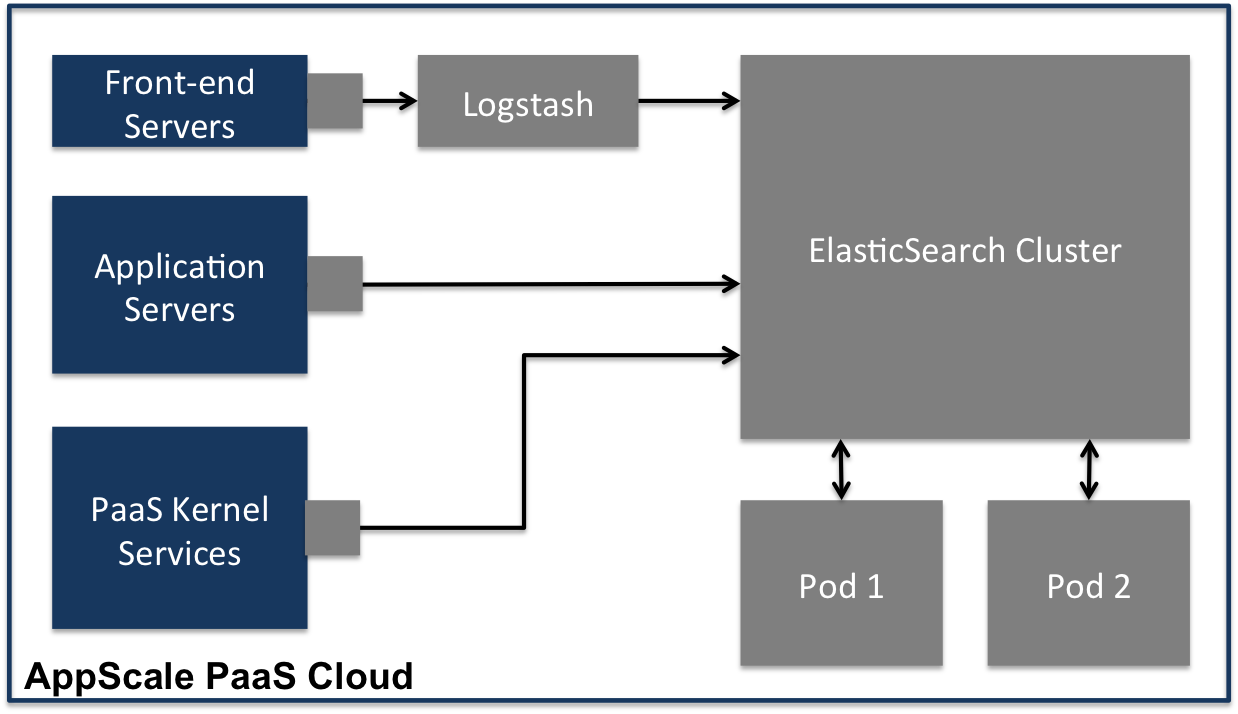
\includegraphics[scale=0.3]{roots_impl}
\caption{Roots prototype implementation for AppScale PaaS.}
\label{fig:roots_impl}
\end{figure}

Figure~\ref{fig:roots_impl} shows an overview of our prototype implementation. Roots components
are shown in grey, while the PaaS components are shown in blue.
We use ElasticSearch~\cite{Kononenko:2014:MMR:2597073.2597091} for data storage in our prototype. 
We configure AppScale's front-end server (Nginx) to tag all incoming application requests
with a unique identifier via a custom HTTP header. 
All data collecting agents in the cloud extract this identifier, and include it as an attribute
in all the events reported to ElasticSearch. This enables our prototype to aggregate events based 
on request IDs.

We implement a number of data collecting agents in AppScale to gather runtime information
from all major components of the PaaS. These agents buffer data locally, and store them in ElasticSearch
in batches. Roots persist events when the buffer accumulates 1MB of data or every 15 seconds, whichever comes
first.  This ensures that the events are promptly reported to the Roots data
storage while keeping the memory footprint of the data collecting agents small and bounded. 
For scraping server logs and storing the extracted entries in ElasticSearch,
our prototype uses Logstash~\cite{logstash}. 
To capture the PaaS kernel invocation data, we augment AppScale's PaaS kernel implementation,
which is derived from the GAE PaaS SDK. Specifically, we implement a Roots agent that monitors
and times all PaaS kernel invocations, and reports them to ElasticSearch. 

We implement Roots pods, which contain more computationally intensive Roots components, 
as standalone Java server processes. We use threads to run benchmarkers,
anomaly detectors, and handlers concurrently within each pod. Pods communicate with ElasticSearch via
a web API, and many of the data analysis tasks such as filtering and aggregation are performed
directly in ElasticSearch.

\subsection{Detecting SLO Violations}

The SLO-based anomaly detector of Roots
allows application developers to specify simple performance SLOs for deployed applications. A
performance SLO is an upper bound on the application response time ($T$), and a probability ($p$)
that the application response time is below the specified upper bound. 
When activated, the detector starts an application benchmarking process within a Roots pod
that periodically measures the response time of the target application. Probes made by the benchmarking 
process are several seconds apart in time (defined by the process sampling rate), 
so as not to degrade application performance.
The detector periodically
analyzes the collected response time measurements to check if the application meets the specified performance
SLO. The detector also accepts a minimum sample count as a parameter. This is the minimum number of 
samples the detector should take before evaluating an SLO.  If the fraction of response time measurements
that are
less than $T$ falls below $p$, the SLO has been violated, and Roots triggers an anomaly event.

To prevent the detector from detecting the same anomaly multiple times, we flush
the detection window upon each SLO violation. A side effect of this is that 
the detector is unable to detect
another violation until the window fills again.
For a sampling rate of 15 seconds and a minimum
sample count of 100, this ``warm up'' period will be 25 minutes.

%\subsection{Path Distribution Anomalies}
%%
%We have implemented a path distribution analyzer and anomaly
%detector in Roots. Its function is to identify recurring sequences of
%PaaS kernel invocations made by an application.
%Each identified sequence corresponds to a path of
%execution through the application code (i.e. a path through the control flow graph of the application). 
%This detector is able to determine the frequency with
%which each path is executed over time. Then, using this information which we term
%a ``path distribution,'' it reports an anomaly when the distribution of call paths
%changes. 
%
%%For each application,
%%a path distribution is comprised of the set of execution paths available in
%%that application, along with the proportion of requests that executed each path.
%%It is an indicator of the type of request workload handled by an application.
%%For example consider a data management application that has a read-only execution path, and a read-write 
%%execution path. If 90\% of the requests execute the read-only path, and the remaining 10\% of the requests
%%execute the read-write path, we may characterize the request workload as read-heavy.
%
%%
%%is another special anomaly detector we implement in Roots. This
%%anomaly detector periodically analyzes the PaaS kernel invocations made by the applications.
%By aggregating the PaaS kernel invocations by application request identifiers, and then sorting them by
%their sequence numbers, this anomaly detector is able to identify the sequence of
%PaaS kernel invocations made by each application request. 
%Each identified invocation sequence corresponds to a path of
%execution through the application code (i.e. a path through the control flow graph of the application). 
%Then the anomaly detector evaluates the number of requests
%that invoked the same PaaS kernel invocation sequence. From that the anomaly detector
%computes the distribution of different execution paths of an application.
 
%Roots path distribution analyzer facilitates computing the path distribution for each application
%with no static analysis, by only analyzing the runtime data gathered from the applications.
%The Roots path distribution analyzer  periodically computes the path distribution for a given application.
%If it detects that the latest path distribution is significantly different from the distributions seen in the 
%past, it triggers an anomaly. This is done by computing the mean request proportion for each path
%(over a sliding window of historical data),
%and then comparing the latest request proportion values against the means. If the latest proportion
%is off by more than $n$ standard deviations from its mean, the detector considers it to be an
%anomaly. The sensitivity of the detector can be configured by changing the value of $n$, which
%defaults to 2. 

%This anomaly detector enables developers to know when the nature of their application request
%workload changes. For example in the previous data management application, if suddenly 90\%
%of the requests start executing the read-write path, the Roots path distribution analyzer will
%detect the change as an anomaly. Similarly it is also able to detect when new paths of execution
%are being invoked by requests (a form of novelty detection).

\subsection{Workload Change Analyzer}

To detect changes in workload, Roots implements a workload change analyzer as an anomaly handler. 
This handler is invoked for every anomaly detected by Roots.
The workload change analyzer determines if an anomaly is due to a change in workload (i.e.
an increase in the application request rate). Roots can report
changes in workload via alerts; PaaS administrators can use such alerts to determine when to
add resources to the system.
Roots subjects anomalies \textit{that are not due to a workload change} to bottleneck
identification.

In contrast to the method described 
in~\cite{Magalhaes:2010:DPA:1906485.1906774,
Magalhaes:2011:RAP:1982185.1982234} which uses correlation between request
latency and workload, our 
workload change analyzer uses change point detection algorithms to identify changes in
the application's request rate. 
Our implementation of Roots supports a number of well known change point
detection algorithms (PELT~\cite{doi:10.1080/01621459.2012.737745}, binary segmentation 
and CL method~\cite{chen1993joint}), any of which can be used to detect level shifts in the
workload size.  For the results in this paper, we use PELT to detect changes in workload.
% Algorithms like PELT favor long lasting shifts (plateaus) in the workload trend, over momentary spikes.
%We expect momentary spikes to be fairly common in workload data. But it's the plateaus that cause
%request buffers to fill up, and consume server-side resources for extended periods of time, thus
%causing noticeable performance anomalies.

\subsection{Bottleneck Identification}

Roots performs bottleneck identification for any performance
anomalies that are triggered by something other than a change in workload.
To enable this, Roots performs multiple analyses over the PaaS performance data that it
collects using full-stack monitoring, without application instrumentation.

PaaS applications 
consist of user code that is executed in one or more application servers,
which makes remote service calls to PaaS kernel services. 
AppScale provides the same kernel services provided by GAE (datastore, memcache,
urlfetch, blobstore, user management etc.).
We consider each PaaS kernel invocation and the code running in the application server as 
separate \textit{components}. Each application request causes one or more components to
execute, and any one of the components can become a bottleneck to cause performance anomalies.  
The purpose of bottleneck identification is to find, across all
the components executed by an application, the one that is most likely to have 
degraded application performance.

Roots tracks the total time and the time spent in individual components for each request, 
and relates them via the formula $T_{total} = T_{X_1} + T_{X_2} + ... + T_{X_n} + r$. 
$T_{total}$ is the total execution time of a request. $T_{X_i}$ is the time spent executing
$X_i$; the $i^{th}$ PaaS kernel invocation.  $r$ is the time spent in the resident
application server executing user code (i.e. the time
spent not executing PaaS services during a request). Roots measures the $T$ values in the platform, and
computes $r$ using this formula. $r$ is not measured directly because doing so would require 
application instrumentation. Given that typical PaaS-hosted web
applications spend most of their time executing platform 
services~\cite{Jayathilaka:2015:RTS:2806777.2806842},
we expect $r \ll T_{X_1} + T_{X_2} + ... + T_{X_n}$ in the common case.

\subsubsection{Selecting Bottleneck Candidates}

Roots employs multiple candidate selection algorithms to identify up to four 
components that are potentially
the bottleneck responsible for the detected anomaly. Our algorithms look for
a variety of inconsistencies and changes in the performance characteristics of 
individual components.  In our prototype, we consider the relative importance of components, 
variations in relative importance, and two 
distributional techniques that distinguish rare events and 
outliers in performance history.

\paragraph*{Relative Importance}
Relative importance~\cite{JSSv017i01} identifies the component that is contributing 
the most towards the variance in the total response time. 
To use it, we regress the kernel calls against the total response time.
That is, for a time window $W$ just prior to the detection of the anomaly, Roots
fits a linear model using linear regression of the form
$T_{total} = T_{X_1} + T_{X_2} + ... + T_{X_n}$
over the per-request performance data in the window.

We omit $r$ since it is typically small.
For cases in which the anomaly occurs in $r$ (e.g. a performance problem in the 
application server or user code), $r$ may
not fit our assumption that $r \ll T_{X_1} + T_{X_2} + ... + T_{X_n}$.  When this
occurs, we assume that $r$ is normally distributed and independent, and filter out
requests from the window for which $r$ is larger than the 0.95 quantile ($r > \mu_r + 1.65\sigma_r$)
to preclude them from skewing the regression. 
We consider the influence of $r$ in other methods described below.

Roots ranks the regressors (i.e. $T_{X_n}$ values) based on their contribution to the variance 
in $T_{total}$.  We use the LMG method~\cite{lmg80} to do so which is resistant to multicollinearity, 
and provides a breakdown of the $R^2$ value of
the regression according to how strongly each regressor influences
the variance of the dependent variable ($T_{total}$).
Roots selects the highest ranked component as a candidate.

\paragraph*{Change in Relative Importance}
The next method selects the most likely candidate by detecting \textit{changes} in relative importance
over time.
This indicates how the variance a component contributes towards the total response time has
changed over time.
For this method, Roots divides the time window $W$ into equal-sized segments,
and computes relative importance for regressors within each segment. 
This results in multiple time series of relative importance values.
We subject each relative importance time series to change point analysis (PELT in our prototype), 
and extract the variable that shows an increase in relative importance, if any.
If such a variable is found, then the component
associated with that variable is considered by Roots as a bottleneck candidate.
The candidate selected by this method represents
a component whose performance has been stable in the past, and has become variable recently.

\paragraph*{High Quantiles}
Roots next analyzes the empirical distributions of $T_{X_k}$ and $r$.
Out of all the available distributions,
we wish to find the one whose quantile values are the largest.
Specifically, we compute a high	
quantile (e.g. 0.99 quantile) for each distribution. The component, whose distribution
contains the largest quantile value
is chosen as another potential candidate for the bottleneck. This component can be considered
as having a high latency in general.

\paragraph*{Tail End Values}
Finally, Roots analyzes each $T_{X_k}$ and $r$ distribution to identify the one 
with the largest tail values with respect to a particular high quantile.
For each tail end value $t$, we compute the metric $P^q_t$. 
This is the percentage difference between $t$ and the
$q$ quantile of the corresponding distribution. We set $q$ to 0.99 in our experiments.
Roots selects the component with the 
distribution that has the largest $P^q_t$ as another potential bottleneck candidate.
This method identifies
candidates that contain rare, high-valued outliers (point anomalies) in their distributions.

\subsubsection{Selecting Among Candidates}
The above four methods may select up to four candidate components for the bottleneck. 
We designate 
the candidate chosen by a majority of methods as the actual bottleneck. A four-way
tie is broken by assigning more priority to the candidate chosen by the relative importance
method.
%We use a simple weighting mechanism to identify the root cause of a bottleneck 
%from the selected candidates. There are at most four candidates to consider.  
%The method assigns 4 points to the component chosen
%by relative importance, and 3 points to all other candidates. 
%We declare the bottleneck component as the one with the largest
%point sum.  This method uses relative importance as the tie-breaker because it
%targets components with consistently high variance, and thus is able to identify
%longer lasting performance issues in the system
%(i.e. collective anomalies~\cite{Chandola:2009:ADS:1541880.1541882}).
%Prior work~\cite{Magalhaes:2011:RAP:1982185.1982234} has shown that 
%regression-based techniques are highly effective in root cause analysis.
